%%
%% CS3631 Phase 2 short paper — ACM Conference Proceedings Primary Article
%% Template (acmart, sigconf format), per course spec (CS3631 - Project -
%% 2026.docx, Sec 12): 4-page limit excluding references.
%%
%% NOTE: placeholder ACM rights/venue fields below are left blank/suppressed
%% since this is a course-internal Moodle submission, not an actual ACM
%% conference registration. Fill in real venue details only if/when this is
%% adapted for an actual ACM venue submission.
%%
\documentclass[sigconf,review]{acmart}

%% Suppress the ACM reference/rights boilerplate — no real DOI/ISBN exists
%% for a course submission.
\settopmatter{printacmref=false}
\renewcommand\footnotetextcopyrightpermission[1]{}
\setcopyright{none}
\acmConference[CS3631 2026]{CS3631 Deep Neural Networks — Course Project}{2026}{}
\acmYear{2026}
\acmDOI{}
\acmISBN{}
\acmBooktitle{}

\usepackage{booktabs}
\usepackage{tikz}
\usetikzlibrary{arrows.meta, positioning}
\usepackage{algorithm}
\usepackage{algpseudocode}

\begin{document}

\title{Explainability-Guided SegFormer for Forest Cover Segmentation Using Attention Consistency Supervision}

\author{Dhinanjaya Fernando}
\affiliation{\institution{CS3631 Group Project}\country{}}

\author{Dinura N. Ginige}
\affiliation{\institution{CS3631 Group Project}\country{}}

\author{Kalana Lakshan}
\affiliation{\institution{CS3631 Group Project}\country{}}

\author{Lasana Pahanga}
\affiliation{\institution{CS3631 Group Project}\country{}}

\author{Chanupa Gurusinghe}
\affiliation{\institution{CS3631 Group Project}\country{}}

\renewcommand{\shortauthors}{Fernando, Ginige, Lakshan, Pahanga, and Gurusinghe}

\begin{abstract}
Vision Transformer (ViT)-based segmentation models achieve strong accuracy,
but their internal attention is typically used only for post-hoc
visualization, not as a supervised training signal. Prior work applying
attention supervision for interpretability has focused on medical imaging
and autonomous-driving domains, while forest/non-forest segmentation from
aerial imagery still treats attention purely as an architectural
feature-refinement mechanism, with interpretability evaluated qualitatively
if at all. We present an explainability-guided SegFormer-B0 architecture
that treats attention as a first-class training target: an
\emph{Attention Consistency Loss} aligns the model's internal attention
with the ground-truth forest mask during training, encouraging the network
to focus on canopy regions rather than roads, shadows, or built structures.
Because SegFormer's encoder uses spatial-reduction attention rather than
standard multi-head self-attention, we adapt Gradient-weighted Attention
Rollout to SegFormer, restricting it to the final encoder stage where
attention is square and token-consistent. We introduce a quantitative
metric, Average Attention--Mask Overlap (AAMO), to evaluate interpretability
numerically rather than only visually. On the full 5{,}108-image dataset
(3576/766/766 split, seed 42, 20 epochs), with $\lambda_2$ set by a
validation sweep, the
proposed method raises AAMO from 0.0334 to 0.7476 ($\sim$22$\times$) relative
to a vanilla SegFormer-B0 baseline trained on the same split, at a modest
segmentation cost (Dice 0.8743$\to$0.8577, IoU 0.7766$\to$0.7508), alongside a
full-scale-trained U-Net baseline (Dice 0.8615, IoU 0.7568) on the same
held-out test set. A complete multi-seed ablation study is ongoing.
\end{abstract}

\begin{CCSXML}
<ccs2012>
   <concept>
       <concept_id>10010147.10010257.10010293.10010294</concept_id>
       <concept_desc>Computing methodologies~Neural networks</concept_desc>
       <concept_significance>500</concept_significance>
   </concept>
   <concept>
       <concept_id>10010147.10010257.10010293.10010321</concept_id>
       <concept_desc>Computing methodologies~Image segmentation</concept_desc>
       <concept_significance>500</concept_significance>
   </concept>
   <concept>
       <concept_id>10010147.10010178.10010224.10010225</concept_id>
       <concept_desc>Computing methodologies~Interpretability and explainability</concept_desc>
       <concept_significance>300</concept_significance>
   </concept>
</ccs2012>
\end{CCSXML}

\ccsdesc[500]{Computing methodologies~Neural networks}
\ccsdesc[500]{Computing methodologies~Image segmentation}
\ccsdesc[300]{Computing methodologies~Interpretability and explainability}

\keywords{semantic segmentation, vision transformers, SegFormer, attention supervision, explainable AI, forest cover mapping, remote sensing}

\maketitle

\section{Introduction}

Semantic segmentation of forest cover from aerial imagery underpins
ecological monitoring, deforestation tracking, and land-use management.
Transformer-based models such as SegFormer~\cite{xie2021segformer} have been
applied to this task for their ability to capture long-range spatial
dependencies, but the great majority of transformer segmentation work,
including recent forest-specific studies~\cite{foresanext2026,ppliteseg2026,attunet2022deforestation},
uses attention purely as an architectural mechanism to improve accuracy,
evaluating explainability only through post-hoc qualitative heatmap
inspection, if at all.

Transformer attention in segmentation models is not explicitly guided
during training and frequently attends to task-irrelevant regions --- roads,
shadows, buildings --- rather than the class of interest, reducing both
accuracy at ambiguous boundaries and the trustworthiness of the model's
explanations. No existing work addresses this specifically for
forest/non-forest segmentation, nor evaluates attention faithfulness
quantitatively in this domain.

This paper makes four contributions: (1) an Attention Consistency Loss that
supervises SegFormer-B0's internal attention against the ground-truth
forest mask during training; (2) an adaptation of Gradient-weighted
Attention Rollout to SegFormer's spatial-reduction attention; (3) AAMO, a
quantitative interpretability metric evaluable alongside standard
segmentation metrics; and (4) a preliminary empirical comparison against
U-Net and vanilla SegFormer-B0 baselines showing that explainability-guided
training substantially improves attention faithfulness at only a modest
segmentation-accuracy cost.

\section{Related Work}

Forest-cover segmentation from aerial and satellite imagery has been
approached almost exclusively as an accuracy problem. U-Net~\cite{ronneberger2015unet}
remains the dominant convolutional baseline, and recent forest-specific
datasets such as the WildUAV forest-inspection
benchmark~\cite{blaga2024wilduav} have focused effort on acquiring larger
and more varied labeled imagery (real and simulated, multiple altitudes and
illumination conditions) to improve segmentation accuracy on models such as
HRNet and PointFlow, without examining what the underlying network attends
to or why. Existing work directly relevant to attention supervision falls
into two families.

\textbf{Attention-as-architecture.} ForResANeXt~\cite{foresanext2026} embeds
lightweight attention in residual blocks for forest/non-forest satellite
segmentation; Attention-Refined PP-LiteSeg~\cite{ppliteseg2026} fuses
multi-branch attention for cross-regional UAV forest segmentation; an
attention-based U-Net~\cite{attunet2022deforestation} adds attention gates
for deforestation mapping on Sentinel-2 imagery. All three use attention
purely as a feature-refinement mechanism improving accuracy --- attention is
never supervised or evaluated as an explanation.

\textbf{Attention-as-explainability.} eX-ViT~\cite{zhang2023exvit}
regularizes ViT attention with an attribute-guided loss for weakly
supervised natural-image classification; TransAttUnet~\cite{chen2022transattunet}
integrates guided attention into a U-Net/Transformer hybrid for medical
segmentation; work on driving models~\cite{guiding2024driving} applies an
explicit attention loss to align attention with task-relevant scene regions.
All three supervise attention as a training signal, but outside the
forest/remote-sensing domain and without a quantitative attention-mask
overlap metric. The attention-extraction method underlying our approach is
Chefer et al.'s Gradient-weighted Attention
Rollout~\cite{chefer2021transformer}, originally defined for standard
multi-head self-attention.

\textbf{Gap.} No prior work combines (a) attention supervision as a
training signal, (b) the forest/non-forest remote-sensing domain, and (c) a
quantitative interpretability metric evaluated alongside standard
segmentation metrics. The attention-as-architecture
literature~\cite{foresanext2026,ppliteseg2026,attunet2022deforestation}
operates in the correct domain but never supervises or measures attention
as an explanation. The attention-as-explainability
literature~\cite{zhang2023exvit,chen2022transattunet,guiding2024driving}
supervises attention as a training signal but never in the
forest-segmentation domain, and none of the three reports a quantitative
attention-fidelity metric comparable across model configurations. This
paper addresses that combined gap: an Attention Consistency Loss that
supervises SegFormer's internal attention against the ground-truth forest
mask, an adaptation of Gradient-weighted Attention Rollout to SegFormer's
spatial-reduction attention, and AAMO, a new quantitative metric that lets
attention fidelity be reported and compared the same way Dice or IoU are.
We also draw on the WildUAV forest inspection dataset
work~\cite{blaga2024wilduav} as evidence that forest-aerial-segmentation
research so far has focused effort on acquiring larger and more varied
labeled imagery rather than on what the resulting models attend to.

\section{Proposed Method}

\subsection{Architecture Overview}
The pipeline (Figure~\ref{fig:pipeline}) extends SegFormer-B0 with an
explainability-supervision path applied during training only; at inference
the model runs as standard SegFormer-B0 with negligible overhead. The
encoder's stage-4 attention (the only stage with spatial-reduction ratio
$=1$, giving square, token-consistent $64\times64$ self-attention) feeds an
adapted Gradient-weighted Attention Rollout to produce attention map $A$.
The ground-truth mask $Y$ is Gaussian-smoothed into a soft target $A^{*}$.
$A$ and $A^{*}$ are compared by the Attention Consistency Loss and combined
with the standard segmentation loss.

\begin{figure}[t]
\centering
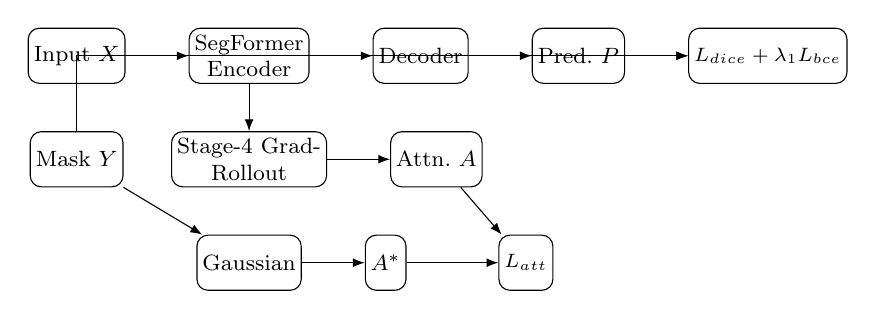
\begin{tikzpicture}[
  node distance=6mm and 8mm,
  box/.style={draw, rounded corners, align=center, minimum height=7mm, font=\footnotesize, inner sep=2pt},
  arr/.style={-{Latex[length=1.5mm]}}
]
\node[box] (x) {Input $X$};
\node[box, right=of x] (enc) {SegFormer\\Encoder};
\node[box, right=of enc] (dec) {Decoder};
\node[box, right=of dec] (p) {Pred.\ $P$};

\node[box, below=of enc] (roll) {Stage-4 Grad-\\Rollout};
\node[box, right=of roll] (a) {Attn.\ $A$};

\node[box, below=of x] (y) {Mask $Y$};
\node[box, below=of roll] (gauss) {Gaussian};
\node[box, right=of gauss] (astar) {$A^{*}$};

\node[box, below right=6mm and 2mm of a, font=\scriptsize] (latt) {$L_{att}$};
\node[box, right=of p, font=\scriptsize] (lseg) {$L_{dice}+\lambda_1 L_{bce}$};

\draw[arr] (x) -- (enc);
\draw[arr] (enc) -- (dec);
\draw[arr] (dec) -- (p);
\draw[arr] (enc) -- (roll);
\draw[arr] (roll) -- (a);
\draw[arr] (y) -- (gauss);
\draw[arr] (gauss) -- (astar);
\draw[arr] (a) -- (latt);
\draw[arr] (astar) -- (latt);
\draw[arr] (p) -- (lseg);
\draw[arr] (y) |- (lseg);
\end{tikzpicture}
\caption{Training pipeline: predicted mask $P$ and attention map $A$ are
each supervised, then combined into the total training objective $L$.}
\label{fig:pipeline}
\end{figure}

\subsection{Handling Spatial-Reduction Attention}
Standard Attention Rollout assumes full multi-head self-attention across all
tokens. SegFormer's Efficient Self-Attention reduces keys/values by a
spatial-reduction ratio at earlier stages (sr $=8,4,2$ for stages 1--3),
making those stages' attention matrices rectangular rather than square.
Only stage 4 (sr $=1$) has true square, token-consistent $64\times64$
attention --- the only stage where Rollout's recursive matrix product is
valid without further approximation, verified empirically on MiT-B0 at
$256{\times}256$ input resolution.

\subsection{Mathematical Formulation}
\label{sec:formulation}
Let $X \in \mathbb{R}^{256\times256\times3}$ and ground-truth mask
$Y \in \{0,1\}^{256\times256}$:
\begin{align}
F &= E(X),\quad P = D(F) \in [0,1]^{256\times256} \\
A &= \mathrm{Rollout}(F) \in [0,1]^{256\times256} \\
A^{*} &= \mathrm{Gaussian}(Y) \\
L_{dice} &= 1 - \frac{2|P\cap Y|}{|P|+|Y|}, \quad
L_{bce} = -\sum \big[Y\log P + (1{-}Y)\log(1{-}P)\big] \\
L_{att} &= \mathrm{MSE}(A, A^{*}) \;\text{or}\; \mathrm{KL}(A \,\|\, A^{*}) \\
L &= L_{dice} + \lambda_1 L_{bce} + \lambda_2 L_{att}
\end{align}
with $\lambda_1{=}1$ and $\lambda_2$ tuned on the validation set: a sweep
over $\lambda_2 \in \{0.1, 0.3, 0.5, 1.0\}$ (MSE, all else fixed) selects
$\lambda_2{=}1.0$, which maximizes test AAMO.
Because $A$ is itself defined via a gradient (Grad-Rollout is
Grad-CAM-style), backpropagating $L_{att}$ requires double backpropagation;
our implementation keeps $A$ attached to the autograd graph via
\texttt{create\_graph=True} so one combined \texttt{backward()} reaches all
parameters.

\begin{algorithm}[t]
\caption{One training step of the attention-consistency variant}
\label{alg:train}
\begin{algorithmic}[1]
\Require image $X$, ground-truth mask $Y$, model $(E, D)$, weights $\lambda_1,\lambda_2$
\State $F \gets E(X)$ \Comment{encoder features, all 4 stages}
\State $P \gets D(F)$ \Comment{decoder segmentation output}
\State $A \gets \mathrm{Rollout}(F_4)$ \Comment{stage-4 attention only, autograd-attached}
\State $A^{*} \gets \mathrm{Gaussian}(Y, \sigma{=}8)$ \Comment{soft attention target}
\State $L \gets L_{dice}(P,Y) + \lambda_1 L_{bce}(P,Y) + \lambda_2 L_{att}(A,A^{*})$
\State $L$.backward(create\_graph=True) \Comment{double backprop: $A$ depends on $\nabla F$}
\State optimizer.step()
\end{algorithmic}
\end{algorithm}

Algorithm~\ref{alg:train} summarizes one training step. At inference, only
lines 1--2 run --- the Rollout/attention path is training-only supervision,
so deployment cost equals vanilla SegFormer-B0.

\subsection{AAMO: Average Attention--Mask Overlap}
Standard practice evaluates attention maps only qualitatively, by visual
inspection of heatmaps. We instead define AAMO to make attention fidelity
reportable and comparable the same way Dice or IoU are. Given normalized
attention $A \in [0,1]^{256\times256}$ and ground-truth mask $Y$, AAMO is the
fraction of forest pixels covered by thresholded attention:
\begin{align}
A_{thr} &= \mathbb{1}[A > \tau], \quad \tau = 0.5 \\
\mathrm{AAMO} &= \frac{|A_{thr} \cap Y|}{|Y|}
\end{align}
i.e.\ AAMO is the recall of the ground-truth forest region under
thresholded attention: 1.0 means attention fully covers the forest mask,
0.0 means no overlap. We additionally report $\mathrm{AAMO_{dice}}$ and
$\mathrm{AAMO_{IoU}}$ (Dice and IoU between $A_{thr}$ and $Y$) as symmetric
overlap checks, since AAMO alone does not penalize attention that also
covers large non-forest regions.

\section{Experimental Setup}
\textbf{Dataset.} 5{,}108 RGB aerial images ($256{\times}256$) with binary
forest/non-forest masks; 70/15/15 stratified train/val/test split. A full
dataset audit confirms 0 orphaned image/mask pairs, 0 unreadable files, and
that masks are already effectively binary --- no pixel sits more than 9 grey
levels from pure black or white, and the mid-gray band (32--223) is empty.
The dataset is moderately forest-majority (mean forest-pixel ratio
$0.6117 \pm 0.3306$ per mask), which we account for by reporting Dice/IoU/F1
rather than pixel accuracy alone, since accuracy alone would be inflated by
the majority class.
U-Net and both SegFormer-B0 variants below are trained and evaluated on the
full 5{,}108-image dataset, using an identical 3576/766/766 split (seed 42)
so all three share the same 766-image held-out test set. DeepLabV3+ remains
a 200-image CPU-scale smoke run, an optional extra reference point pending a
full-scale run.

\textbf{Baselines.} U-Net (CNN) and vanilla SegFormer-B0 (no attention
loss), isolating the effect of the proposed attention supervision, plus
DeepLabV3+ (MobileNetV3 backbone) as an additional optional CNN reference
point.

\textbf{Metrics.} Dice, IoU, F1 (segmentation quality); parameter count,
GFLOPs, FPS (efficiency); AAMO --- normalized overlap between thresholded
attention and the ground-truth forest mask (interpretability).

\textbf{Implementation details.} SegFormer-B0 variants are trained on a GPU
runtime for 20 epochs with AdamW (lr $=6{\times}10^{-5}$), batch size 16
(vanilla) / 1 (attention variant, due to the double-backpropagation memory
cost), Gaussian target smoothing $\sigma = 8$, and $L_{att}$ using the MSE
formulation, seed 42. The attention-loss weight is set to $\lambda_2 = 1.0$,
the value selected by the validation sweep (Section~\ref{sec:formulation}).
Reported checkpoints are each variant's best-validation epoch (vanilla:
epoch 5; attention-consistency: epoch 11) rather than the final epoch, since
training Dice reaches $\sim$0.90 by epoch 20 while validation Dice peaks
earlier. Both the MSE and KL-divergence
formulations of $L_{att}$ are implemented and unit-tested, but only MSE has
been evaluated on trained checkpoints so far.

\textbf{Reproducibility.} The attention-extraction and loss implementation
is covered by 13 unit tests independent of any trained model (8 for the
Attention Consistency Loss, 5 verifying Grad-Rollout output shapes at each
SegFormer stage), and AAMO by 10 further tests on synthetic
attention/mask pairs, all passing. Dataset integrity is checked by a
standalone auditing script (pairing, geometry, value spread, class balance)
that exits non-zero on failure, so it can run as a pre-flight gate before
training rather than being assumed correct.

\section{Results}

Table~\ref{tab:results} reports the full 5{,}108-image, 20-epoch GPU run for
U-Net and both SegFormer-B0 variants (attention variant: $\lambda_2{=}1.0$),
all on the same 3576/766/766 held-out test set. AAMO increases approximately
$22\times$ (0.0334 $\to$ 0.7476) with the attention-consistency variant, at a
modest cost in Dice (0.8743$\to$0.8577). Across the
$\lambda_2$ sweep (0.1--1.0, MSE), test AAMO rises monotonically (0.548,
0.575, 0.603, 0.748) while test Dice stays within 0.852--0.869.
Our earlier 400/60/60, 8-epoch CPU smoke run had instead shown the attention
loss slightly \emph{improving} Dice/IoU
(0.8017$\to$0.8191, 0.6690$\to$0.6936); that small-scale accuracy gain did
not hold at full scale, though the AAMO direction was consistent at both
scales (smoke: 0.0144$\to$0.432). We additionally report
DeepLabV3+ (MobileNetV3 backbone) as an optional CNN reference point beyond
U-Net; on a 200-image smoke run it trails both U-Net and SegFormer-B0 on
Dice/IoU and shows a strong precision/recall imbalance (precision 0.59,
recall 0.98), indicating a bias toward over-predicting forest rather than
delineating boundaries precisely.

\begin{table}[t]
\caption{Comparison on the full 5{,}108-image dataset (3576/766/766 split,
seed 42): U-Net and SegFormer-B0 variants share this held-out test set. The
attention-consistency row uses $\lambda_2{=}1.0$, selected by a validation
sweep over $\{0.1, 0.3, 0.5, 1.0\}$; checkpoints are each variant's
best-validation epoch (vanilla 5, attention-consistency 11). DeepLabV3+
remains a 200-image smoke run, an optional extra baseline not yet run at
full scale.}
\label{tab:results}
\begin{tabular}{@{}lccc c@{}}
\toprule
Model & Dice & IoU & F1 & AAMO \\
\midrule
U-Net (CNN) & 0.8615 & 0.7568 & 0.8615 & n/a \\
DeepLabV3+ (MobileNetV3) & 0.7369 & 0.5834 & 0.7369 & n/a \\
SegFormer-B0 & 0.8743 & 0.7766 & 0.8743 & 0.0334 \\
SegFormer-B0 + $L_{att}$ & 0.8577 & 0.7508 & 0.8577 & \textbf{0.7476} \\
\bottomrule
\end{tabular}
\end{table}

\begin{figure*}[t]
\centering
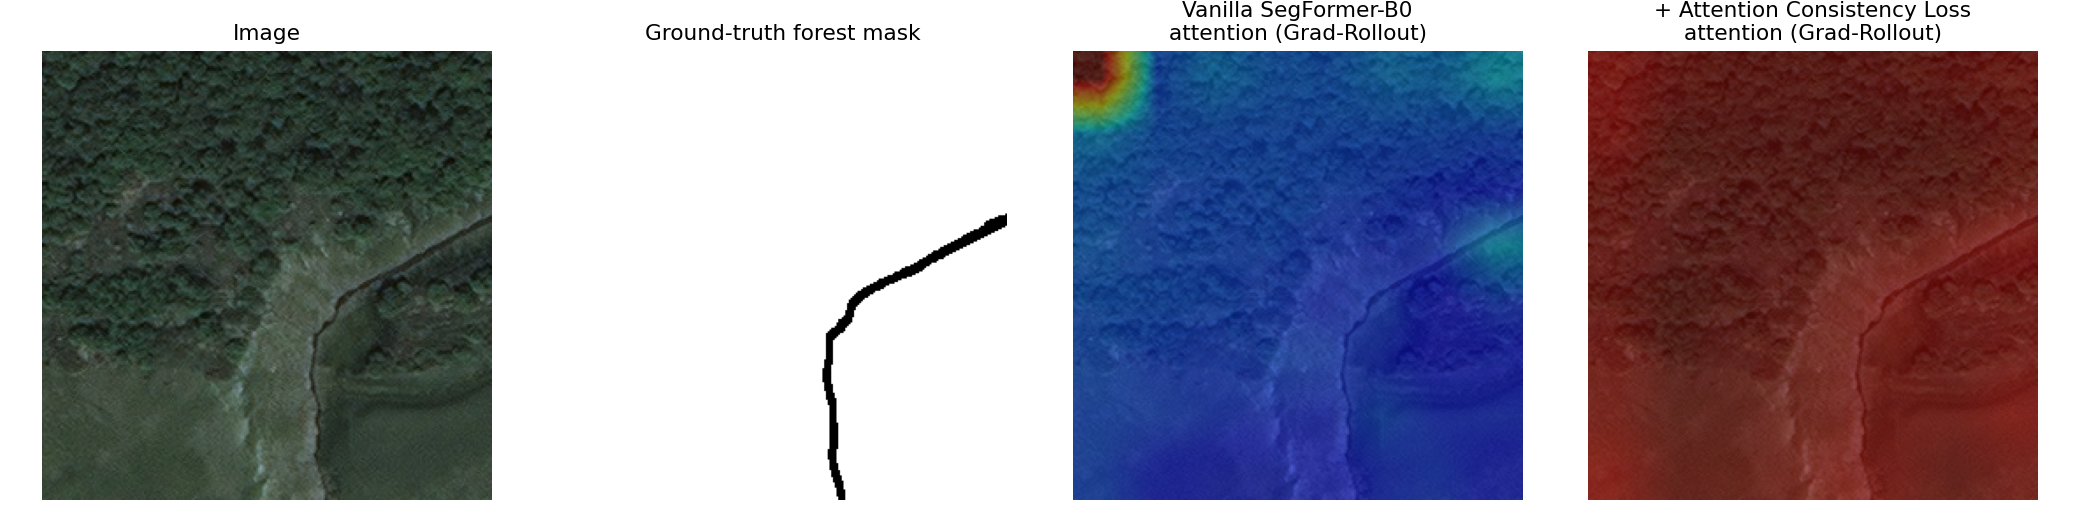
\includegraphics[width=\textwidth]{figures/attention_drift_01_full_scale.png}
\caption{Qualitative comparison on a held-out test image (left to right):
input image; ground-truth forest mask; vanilla SegFormer-B0 attention
(Grad-Rollout); attention after adding the Attention Consistency Loss
($\lambda_2{=}0.3$ checkpoint; $\lambda_2{=}1.0$ map pending).
Full-scale checkpoints (5{,}108 images, 20 epochs, best-val). The
attention-consistency map shifts attention broadly toward the darker canopy
clusters and away from the bare ground, consistent with the AAMO gain, but
still does not cleanly separate canopy from non-forest by eye. The vanilla
model's attention remains dominated by corner/edge hot spots rather than the
motivating roads/shadows failure mode even at full scale, indicating this is
not simply an undertraining artifact as earlier speculated from the
8-epoch smoke run. Genuine output of the trained checkpoints; one of three
qualitative comparisons generated, not otherwise cherry-picked.}
\label{fig:attn}
\end{figure*}

\textbf{Augmentation ablation (U-Net, full scale).} Separately from the
smoke-scale numbers above, a full-scale (5{,}108-image, 20-epoch)
augmentation ablation on the U-Net baseline --- same split, seed, and
starting weights, toggling only the augmentation pipeline --- finds that
augmentation does not improve accuracy under this training budget: test
Dice falls from 0.8604 (no augmentation) to 0.8505 (with augmentation),
IoU from 0.7598 to 0.7454. Neither arm overfits within 20 epochs, the
regime in which augmentation is expected to pay off, and this is a
single-seed result, so we read it as \emph{augmentation did not improve
the U-Net baseline under our training budget}, not as evidence that
augmentation is unhelpful for this task in general.

\textbf{Remaining limitations.} The full 5{,}108-image, 20-epoch run
resolves the earlier smoke-scale caveat for U-Net and both SegFormer-B0
variants, but the SegFormer checkpoints are still early-stopped at their
best-validation epoch rather than fully converged, the $\lambda_2$ sweep is
single-seed, and no run has yet been repeated with a different seed.
DeepLabV3+ remains a 200-image
smoke-scale reference only. Figure~\ref{fig:attn} shows the qualitative
attention-drift comparison still does not tell as clean a story as the AAMO
number: the vanilla model's attention continues to exhibit a corner/edge
artifact rather than the motivating roads/shadows failure mode, and this
persists at full scale, so it is unlikely to be simply an undertraining
effect as earlier speculated.

\section{Discussion}
The large AAMO gain relative to a small Dice/IoU reduction suggests
attention faithfulness and segmentation accuracy are, at least partially,
separable objectives: the $\lambda_2$ sweep's monotonic AAMO trend with a
near-flat Dice band indicates a tunable trade-off, not a sharp accuracy
collapse. This now holds at full scale (5{,}108
images, 20 epochs) as well as at the earlier smoke scale, though a
multi-seed ablation is still required before drawing firm conclusions. Both
the MSE and KL-divergence formulations of $L_{att}$ are implemented; only
MSE has been evaluated so far.

\textbf{Threats to validity.} (1) \emph{Scale.} U-Net and both SegFormer-B0
variants are now trained and evaluated on the full 5{,}108-image dataset for
20 epochs, sharing the same 766-image held-out test set, resolving this
threat for those three rows; DeepLabV3+ remains a 200-image smoke-scale
reference only, so its comparison to the other rows should be read with that
caveat. The SegFormer checkpoints are early-stopped at their best-validation
epoch rather than fully converged. (2) \emph{Single seed.} No run has been
repeated with a different seed, and the $\lambda_2$ sweep that selects
$\lambda_2{=}1.0$ is itself single-seed, so the reported numbers carry
unknown variance; Phase 2's multi-seed ablation is required before any
number here is treated as final.
(3) \emph{CNN baseline provenance.} The reported U-Net baseline is now the
PyTorch model trained with the identical split, seed, and training loop as
the SegFormer runs (resolved from an earlier draft that mixed in a
separately-trained Keras model); Dice/IoU are computed dataset-wide
(TP/FP/FN accumulated over all 766 test images), consistent with how the
other rows in Table~\ref{tab:results} are computed. (4) \emph{Rollout
restriction.}
Restricting Gradient-weighted Attention Rollout to SegFormer's stage-4
attention avoids the invalid rectangular-matrix case but discards
information from stages 1--3, which this work does not yet quantify the
cost of. (5) \emph{Boundary loss / attention interaction.} A preliminary
Phase 2 sweep of the boundary-refinement loss weight $\lambda_3 \in
\{0.1, 0.2, 0.5\}$ (fixed at the $\lambda_2{=}1.0$ winner) finds AAMO drops
non-monotonically as $\lambda_3$ increases (0.7775, 0.6218, 0.6805 against
the $\lambda_3{=}0$ baseline's 0.7476) even as test Dice improves (up to
0.8669 at $\lambda_3{=}0.2$). Best-validation checkpoints for
$\lambda_3{\ge}0.2$ are selected far earlier in training (epoch 4) than the
$\lambda_3{\in}\{0,0.1\}$ runs (epoch 11), consistent with $L_{boundary}$'s
gradient --- which flows through the same shared encoder that produces the
attention maps --- competing with $L_{att}$ for representation capacity;
this is single-seed evidence at batch size 1 and not yet disentangled from
checkpoint-selection noise.

\textbf{Broader impact.} Forest-cover monitoring increasingly informs
deforestation-tracking and conservation-policy decisions, where an
automated model's \emph{explanation} of a prediction --- not just its
accuracy --- affects whether domain experts and policymakers can trust it.
An attention map that reliably attends to canopy rather than roads or
shadows is a step toward auditable forest monitoring, but these preliminary,
single-seed results are not yet reliable enough to inform real
deforestation-monitoring decisions.

\section{Conclusion and Future Work}
We presented an explainability-guided SegFormer-B0 that supervises internal
attention against the ground-truth forest mask via an Attention Consistency
Loss, an adaptation of Gradient-weighted Attention Rollout to SegFormer's
spatial-reduction attention, and a new quantitative interpretability
metric, AAMO. Full-scale results on the 5{,}108-image dataset confirm the
core hypothesis: with $\lambda_2{=}1.0$ (validation-swept), AAMO rises
$\sim$22$\times$ (0.0334$\to$0.7476) for a $\sim$1.7-point Dice cost. Future
work will run the complete multi-seed ablation study, compare the MSE and
KL-divergence loss formulations, extend the $\lambda_2$ sweep to multiple
seeds, address the residual overfitting, and, time permitting, add a
boundary-refinement module targeting canopy-edge errors.

\bibliographystyle{ACM-Reference-Format}
\bibliography{references}

\end{document}
